\documentclass[compress,11pt]{beamer}

\usetheme{TALK}
\usepackage[vcentermath]{genyoungtabtikz}
\usepackage{minted}
\usemintedstyle{emacs}
\usepackage{tikz}\usetikzlibrary{trees}
\usepackage{xspace}

\usemintedstyle{emacs}
%\usemintedstyle{colorful}
%\usemintedstyle{borland}
%\usemintedstyle{autumn}

%\newminted{coq}{
%frame=lines,
%framesep=2mm,
%fontsize=\scriptsize,
%mathescape=true
%}
\usepackage{commath}

% INFO DOCUMENT - TITRE, AUTEUR, INSTITUTION
\title{\bf\LARGE HPC en Combinatoire :  \\
Applications du vol de tâches\\[5mm]}
%\subtitle{}
\author{Florent Hivert}
\institute[LRI]{
  LRI / Université Paris Sud 11 / CNRS}
\date[Décembre 2014]{Mars 2015}

\newcommand{\XX}{{\mathbb X}}

\newcommand{\free}[1]{\left\langle#1\right\rangle}
\newcommand{\N}{{\mathbb N}}
\newcommand{\C}{{\mathbb C}}
\newcommand{\Q}{{\mathbb Q}}
\newcommand{\SG}{{\mathfrak S}}
\newcommand{\std}{\operatorname{Std}}

\newcommand{\sym}{\mathrm{sym}}
\newcommand{\NCSF}{\mathbf{NCSF}}
\newcommand{\QSym}{\mathrm{QSym}}
\newcommand{\FSym}{\mathbf{FSym}}

\newcommand{\partof}{\vdash}                    % Partition de
\newcommand{\compof}{\vDash}                    % Composisition de

\newcommand{\qandq}{\text{\quad et\quad}}

\newcommand{\alphX}{{\mathbb X}}

%%%%%%%%%%%%%%%%%%%%%
%\renewcommand{\emph}[1]{{\color{red} #1}}
%------------------------------------------------------------------------------
\begin{document}

% PAGE D'ACCUEIL
\frame{\titlepage}

\begin{frame}{Outline}

  \tableofcontents
\end{frame}


\section{Background: Sage/OpenDreamKit/HPC in Combinatorics}
\begin{frame}{The \textbf{SageMath} system}

  \centering
  \url{www.sagemath.org}
  \bigskip

  \textbf{SageMath} is a {\color{green} free open-source mathematics software}
  system licensed under the GPL. It builds on top of many existing open-source
  packages: NumPy, SciPy, matplotlib, Sympy, Maxima, GAP, FLINT, R and many
  more. Access their combined power through a common, {\color{green}
    Python}-based language or directly via interfaces or wrappers.  \bigskip

  Mission: \textbf{«Creating a {\color{red} viable free open source
      alternative} to Magma, Maple, Mathematica and Matlab.»}
\end{frame}

\begin{frame}[fragile]{The OpenDreamKit project}

  \textbf{\Large Open Digital Research Environment Toolkit for the
    Advancement of Mathematics}
  \begin{itemize}
  \item Horizon 2020, European Research Infrastructures, Work Program
    Call: Virtual Research Environments
  \item 15 sites, 50 participants
  \end{itemize}
  {\color{red} Goals} (see {\color{blue}\url{http://opendreamkit.org/}} for details):
  \begin{itemize}
  \item \textbf{Foster the ecosystem} of open source software for pure
    mathematics and beyond
  \item Deliver a \textbf{flexible Virtual Research Environment toolkit} supporting
    collaborative work on \emph{software}, \emph{data}, and \emph{knowledge}
  \item \textbf{Sustain long term viability} by outsourcing components or
    joining forces with the wider community whenever possible
  \end{itemize}
\end{frame}

\begin{frame}{The Sage-Combinat project}

  \centering
  \url{http://wiki.sagemath.org/combinat}
  \bigskip

  \textbf{Sage-Combinat} is a software project whose mission is: 

  \textbf{«to improve
    the open source mathematical system Sage as an extensible toolbox for
    computer exploration in (algebraic) combinatorics, and foster code sharing
    between researchers in this area.»}
  \bigskip

  50~contributors, 1200+ ticket.
\end{frame}


%%%%%%%%%%%%%%%%%%%%%%%%%%%%%%%%%%%%%%%%%%%%%%%%%%%%%%%%%%%%%%%%%%%%%%%%%%%%%
\begin{frame}[fragile]{Algebraic combinatorics}

Liens profonds
$$\fbox{\parbox{3cm}{\centering comportement des algorithmes}}
 \quad\Longleftrightarrow\quad
\fbox{\parbox{1.8cm}{\centering identités algébriques}}$$
\medskip

Calcul algébrique
{\textbf{à l'aide de / sur les / objets combinatoires}}%
$$
(()(()())(()))(()())
\qquad
  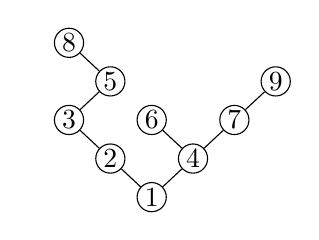
\begin{tikzpicture}[baseline=(current bounding box.center), scale=0.7, inner
    sep=0.3mm, % distance from a label to its surrouding circle
    level distance=7mm % distance between two levels
%    ,edge from parent/.style={<-,draw}
   ]
    \node[circle, draw] {1} [grow'=up]
        child {node[circle, draw] {2}
           child{node[circle,draw] {3}
             child{ {} edge from parent[draw=none]}
             child{node[circle,draw] {5}
               child{node[circle,draw] {8}}
               child{ {} edge from parent[draw=none]}
             }
           }
           child{ {} edge from parent[draw=none]}
        }
        child {node[circle, draw] {4}
           child{node[circle,draw] {6}}
           child{node[circle,draw] {7}
             child{ {} edge from parent[draw=none]}
             child{node[circle,draw] {9}}
           }
        }
    ;
  \end{tikzpicture}
\qquad
\young(5,269,13478)
%\Tableau{c & e \\ b & d & d \\ a & a & b & c \\}
$$

Les structures récursive des objets combinatoires reflètent les structures
algébriques.
\end{frame}
%%%%%%%%%%%%%%%%%%%%%%%%%%%%%%%%%%%%%%%%%%%%%%%%%%%%%%%%%%%%%%%%%%%%%%%%%%%%%
\begin{frame}{Algebraic combinatorics}

\[\includegraphics[width=11cm]{mindmap.pdf}\]
\end{frame}
%%%%%%%%%%%%%%%%%%%%%%%%%%%%%%%%%%%%%%%%%%%%%%%%%%%%%%%%%%%%%%%%%%%%%%%%%%%%%
\begin{frame}{Algebraic combinatorics : experimental mathematics}

A very large range of tools mathematical tools are needed:
\begin{itemize}
\item Manipulation of combinatorial objects:
  \begin{itemize}
  \item integer partitions, set partitions, permutations, trees, \dots
  \item words, language, automatons, \dots
  \item relations, graphs, partial orders, \dots
  \end{itemize}
\item fast exact linear algebra over various rings
\item commutative or not algebra (polynomials, series, \dots)
\item advanced algebraic computations (groups, group algebra, modules \dots).
\end{itemize}
\bigskip\pause

Together with a very good language support:
\begin{itemize}
\item Advanced programming concept (objects, aspect \dots).
\item basic persistent data structures
\item multicore, distributed computation
\item databases
\end{itemize}
\end{frame}

%%%%%%%%%%%%%%%%%%%%%%%%%%%%%%%%%%%%%%%%%%%%%%%%%%%%%%%%%%%%%%%%%%%%%%%%%%%%%
\begin{frame}{Algebraic combinatorics : experimental mathematics}

\textbf{\Large We code primarily for research}
\begin{itemize}
\item rapid prototyping
\item $90\%$ of the code is thrown away
\bigskip\pause
\item need high level, expressive language and libraries
\item the language of the code should be as close as possible to maths
\end{itemize}
\bigskip\pause
\textbf{\Large Combinatorial explosion}
\begin{itemize}
\item We need the code to be reasonably efficient
\item Everything which allows to speed-up high level code is good !
\end{itemize}
\end{frame}

%%%%%%%%%%%%%%%%%%%%%%%%%%%%%%%%%%%%%%%%%%%%%%%%%%%%%%%%%%%%%%%%%%%%%%%%%%%%%
\section{Recursively enumerated sets (RESets)}
%%%%%%%%%%%%%%%%%%%%%%%%%%%%%%%%%%%%%%%%%%%%%%%%%%%%%%%%%%%%%%%%%%%%%%%%%%%%%
\begin{frame}[fragile]{Today: Map/Reduce of RESets}

  \begin{center}
    \shadowbox{%
      \begin{minipage}{8cm}\large\bf
        Perform a Map/Reduce operation on a very large set described
        recursively.
      \end{minipage}
    }
  \end{center}
  \bigskip\pause

  \begin{itemize}
  \item Typically the sets doesn't fit in the computer memory.
    \medskip

  \item Compute the cardinality
  \item Compute any kind of generating series
  \item Test a conjecture : i.e. find an element of $S$ satisfying a specific
    property, or check that all of them do
  \item Count/list the elements of $S$ having this property
  \end{itemize}
\end{frame}

\begin{frame}[fragile]{Today: Map/Reduce of RESets}

  \textbf{Inputs}:
  \bigskip

  A \textbf{recursively enumerated set}
  \begin{itemize}
  \item the \texttt{roots} of the recursion
  \item the \texttt{children} function
  \item the \texttt{postprocessing} function
  \end{itemize}
  A \textbf{Map/Reduce problem}
  \begin{itemize}
  \item the \texttt{mapped} function
  \item the \verb|reduce_init| function
  \item the \texttt{reduce} function
  \end{itemize}
\end{frame}

\begin{frame}[fragile]{Recursively enumerated sets (RESets)}
\newcommand{\sgnode}[1]{{\bf \left<#1\right>}}
\newcommand{\gr}[1]{{\color{gray} #1}}

The tree of numerical semigroups
\tiny
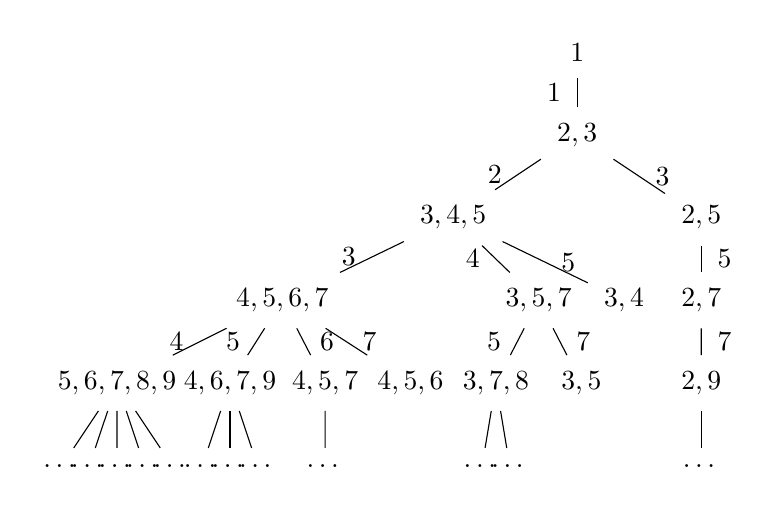
\begin{tikzpicture}[baseline={([yshift=-5cm]current bounding box.north)},
  scale=0.7,
  level distance=1.5cm, 
  inner sep=2mm,
  level/.style={sibling distance=1.55cm}]
    \node {$\sgnode{1}$}
    child {node {$\sgnode{2,3}$}
      child [sibling distance=4.5cm] {node {$\sgnode{3,4,5}$}
        child {node {$\sgnode{4,5,6,7}$}
          child [sibling distance=2cm]{node {$\sgnode{5,6,7,8,9}$}
            child[sibling distance=0.5cm] {node {$\dots$} edge from parent}
            child[sibling distance=0.5cm] {node {$\dots$} edge from parent}
            child[sibling distance=0.5cm] {node {$\dots$} edge from parent}
            child[sibling distance=0.5cm] {node {$\dots$} edge from parent}
            child[sibling distance=0.5cm] {node {$\dots$} edge from parent}
            edge from parent node [left] {4}}
          child [sibling distance=1.9cm]{node {$\sgnode{\gr 4,6,7,9}$}
            child[sibling distance=0.5cm] {node {$\dots$} edge from parent}
            child[sibling distance=0.5cm] {node {$\dots$} edge from parent}
            child[sibling distance=0.5cm] {node {$\dots$} edge from parent}
            edge from parent node [left] {5}}
          child {node {$\sgnode{\gr 4,\gr 5,7}$}
            child[sibling distance=0.5cm] {node {$\dots$} edge from parent}
            edge from parent node [right] {6}}
          child {node {$\sgnode{\gr 4,\gr 5,\gr 6}$}
            edge from parent node [right] {7}}
          edge from parent node [left] {3}
        }
        child{{} edge from parent[draw=none]}
        child{{} edge from parent[draw=none]}
        child {node {$\sgnode{\gr 3,5,7}$}
          child {node {$\sgnode{\gr 3,7,8}$}
            child[sibling distance=0.5cm] {node {$\dots$} edge from parent}
            child[sibling distance=0.5cm] {node {$\dots$} edge from parent}
            edge from parent node [left] {5}}
          child {node {$\sgnode{\gr 3,\gr 5}$} edge from parent node [right] {7}}
          edge from parent node [left] {4}
        }
        child {node {$\sgnode{\gr 3,\gr 4}$}
          edge from parent node [right] {5}
        }
        edge from parent node [left] {2}
      }
      child [sibling distance=4.5cm] {node {$\sgnode{\gr2,5}$}
        child {node {$\sgnode{\gr2,7}$}
          child {node {$\sgnode{\gr2,9}$}
            child[sibling distance=0.5cm] {node {$\dots$} edge from parent}
            edge from parent node [right] {7}
          }
          edge from parent node [right] {5}
        }
        edge from parent node [right] {3}
      }
      edge from parent node [left] {1}
    }
    ;
  \end{tikzpicture}
\end{frame}



%%%%%%%%%%%%%%%%%%%%%%%%%%%%%%%%%%%%%%%%%%%%%%%%%%%%%%%%%%%%%%%%%%%%%%%%%%%%%
\section{The problem: Map/Reduce on RESets}
%%%%%%%%%%%%%%%%%%%%%%%%%%%%%%%%%%%%%%%%%%%%%%%%%%%%%%%%%%%%%%%%%%%%%%%%%%%%%

\begin{frame}[fragile]{Map/Reduce on RESets}

\begin{minted}{python}
sage: S = RecursivelyEnumeratedSet(
....:   [[]],
....:   lambda l: [l+[0], l+[1]] if len(l) <= 15 else [],
....:   structure='forest', enumeration='depth')
sage: S.map_reduce(
....:   map_function = lambda x: 1,
....:   reduce_function = lambda x,y: x+y,
....:   reduce_init = 0 )
131071
\end{minted}
\end{frame}



\section{A Python Implementation of Map/Reduce on RESets}

\begin{frame}[fragile]{Parallelism in Python}

\textbf{CPython has a Global interpreter lock (GIL) !}
\bigskip

\begin{itemize}
\item No Parallel thread execution
  \begin{itemize}
  \item Note: Python's GC uses reference counting, therefore the destructor
    \verb+__del__+ isn't thread-safe
  \item Note: it is possible to release the GIL in C modules
  \end{itemize}
\end{itemize}

\pause
\textbf{Solution:}
\begin{itemize}
\item multiprocess with several Python interpreters with IPC
\item serialization (pickling in Python's dialect)
\item Uses the \texttt{multiprocessing module}
\end{itemize}

\end{frame}

\begin{frame}{Implantation en Python utilisant multiprocessing}

\end{frame}

\begin{frame}{Work-Stealing System Architecture}

\[\hspace{-0.7cm}\includegraphics[width=12.5cm]{scheme.pdf}\]
\end{frame}

\begin{frame}[fragile]{Work Stealing: main loop}
\begin{minted}{python}
try:
    while True:
        try:
            node = self._todo.pop()
        except IndexError:
            node = self.steal()
        self.walk_branch_locally(node)
        if self._reduce_locally != True:
            self.send_partial_result()
except AbortError:
    logger.debug("Aborted !")
    results.put(self._res)
\end{minted}
\end{frame}

\begin{frame}[fragile]{Work Stealing: steal loop}
\begin{minted}{python}
self._mapred._signal_task_done()
node = None
while node is None:
    victim = self._mapred.random_worker()
    if victim is not self:
        victim._request.put(self._iproc)
        node = self._read_task.recv()
        if node is AbortError:
            raise AbortError
return node
\end{minted}
\end{frame}

\begin{frame}[fragile]{Vol de Tâches: thief loop}
\begin{minted}{python}
for ireq in iter(self._request.get, AbortError):
    target = self._mapred._workers[ireq]
    self._mapred._signal_task_start()
    try:
        work = self._todo.popleft()
    except IndexError:
        target._write_task.send(None)
        self._mapred._signal_task_done()
    else:
        target._write_task.send(work)
\end{minted}
\end{frame}

\section{HPC with Cilk/SIMD}


\newcommand{\CilkP}{\texttt{Cilk++}\xspace}
\newcommand{\CPP}{\texttt{C++}\xspace}
\newcommand{\MMX}{\texttt{MMX}\xspace}
\newcommand{\SIMD}{\texttt{SIMD}\xspace}
\newcommand{\SSE}{\texttt{SSE}\xspace}
\newcommand{\SSEV}{\texttt{SSE4.1}\xspace}

\begin{frame}[fragile]{When we really need speed !}

  \textbf{Cython:} \textbf{optimising static compiler} for both
  \textbf{Python} and extended Cython programming language.

\begin{itemize}
\item write Python code that calls back and forth from and to C or C++ code
  natively at any point.
\item easily tune readable Python code into plain C performance by adding
  \textbf{static type declarations}.
\end{itemize}
\bigskip\pause

\textbf{Cilk: multithreaded parallel computing}
\begin{itemize}
\item based on the C and C++ programming languages
\item constructs to express parallel loops and the fork–join idiom.
\end{itemize}
\bigskip\pause

\centering \textbf{\Large\color{red}Cilk extensions module for Python/Sage}
\end{frame}

\begin{frame}[fragile]{When we really need speed !}
\begin{itemize}

\item Vectorization (\MMX, \SSE instructions sets) and careful memory alignment;
\item Shared memory multi-core computing using \CilkP for low level
  enumerating tree branching;
\item Partially derecursived algorithm using a stack;
\item Avoiding all dynamic allocation during the computation: everything is
  computed ``in place'';
\item Avoiding all unnecessary copy: Indirection in the stack.
\item Aggressive loop unrolling: the main loop is unrolled by hand using some
  kind of Duff's device;
\item Careful choice of data type (\verb|uint_fast8_t| for decomposition
  number, vs \verb|uint_fast64_t| for all indexes).
\end{itemize}  
\end{frame}

\begin{frame}[fragile]{The results !}

$16$~days on a AMD Opteron(TM) Processor $6276$, $2.3Gz$ using 32~cores.

\tiny
\begin{center}
\begin{tabular}{|r|r||r|r||r|r|}
\hline
g & $n_g$ & g & $n_g$ & g & $n_g$ \\
\hline
0 & 1 & 23 & 170\,963 & 46 & 14\,463\,633\,648\\
1 & 1 & 24 & 282\,828 & 47 & 23\,527\,845\,502\\
2 & 2 & 25 & 467\,224 & 48 & 38\,260\,496\,374\\
3 & 4 & 26 & 770\,832 & 49 & 62\,200\,036\,752\\
4 & 7 & 27 & 1\,270\,267 & 50 & 101\,090\,300\,128\\
5 & 12 & 28 & 2\,091\,030 & 51 & 164\,253\,200\,784\\
6 & 23 & 29 & 3\,437\,839 & 52 & 266\,815\,155\,103\\
7 & 39 & 30 & 5\,646\,773 & 53 & 433\,317\,458\,741\\
8 & 67 & 31 & 9\,266\,788 & 54 & 703\,569\,992\,121\\
9 & 118 & 32 & 15\,195\,070 & 55 & 1\,142\,140\,736\,859\\
10 & 204 & 33 & 24\,896\,206 & 56 & 1\,853\,737\,832\,107\\
11 & 343 & 34 & 40\,761\,087 & 57 & 3\,008\,140\,981\,820\\
12 & 592 & 35 & 66\,687\,201 & 58 & 4\,880\,606\,790\,010\\
13 & 1\,001 & 36 & 109\,032\,500 & 59 & 7\,917\,344\,087\,695\\
14 & 1\,693 & 37 & 178\,158\,289 & 60 & 12\,841\,603\,251\,351\\
15 & 2\,857 & 38 & 290\,939\,807 & 61 & 20\,825\,558\,002\,053\\
16 & 4\,806 & 39 & 474\,851\,445 & 62 & 33\,768\,763\,536\,686\\
17 & 8\,045 & 40 & 774\,614\,284 & 63 & 54\,749\,244\,915\,730\\
18 & 13\,467 & 41 & 1\,262\,992\,840 & 64 & 88\,754\,191\,073\,328\\
19 & 22\,464 & 42 & 2\,058\,356\,522 & 65 & 143\,863\,484\,925\,550\\
20 & 37\,396 & 43 & 3\,353\,191\,846 & 66 & 233\,166\,577\,125\,714\\
21 & 62\,194 & 44 & 5\,460\,401\,576 & 67 & 377\,866\,907\,506\,273\\
22 & 103\,246 & 45 & 8\,888\,486\,816 & &\\
\hline
\end{tabular}
\end{center}
\end{frame}


\end{document}
% "latex -synctex=1 -shell-escape"
%%% Local Variables: LaTeX-command
%%% mode: latex
%%% TeX-master: t
%%% End: 
